\documentclass[10pt,a4paper]{article}
\usepackage[margin=1in]{geometry}
\usepackage{hyperref}
\usepackage{xcolor}
\usepackage{graphicx}

\newcommand{\figref}[1]{Fig. \ref{#1}}
\newcommand{\tabref}[1]{Table \ref{#1}}
\newcommand{\lstref}[1]{Listing \ref{#1}}
\newcommand{\secref}[1]{Section \ref{#1}}
\newcommand{\appref}[1]{Appendix \ref{#1}}
\newcommand{\todo}[1]{{\colorbox{red}{\bf TODO:}\textcolor{red}{#1}}}


\title{PRISM protocol v0.3} 

\author{Atala PRISM team - IOG} 

\date{} 

\begin{document}


\maketitle 

\begin{abstract} 
This document describes the current state of the protocol that supports PRISM. PRISM is a framework for the management of decentralized identifiers and verifiable credentials. 
\end{abstract}

\setcounter{tocdepth}{3} 

\tableofcontents 
\newpage 

%----------------------------------------------------------------------------------------
%	INTRODUCTION
%----------------------------------------------------------------------------------------

\section{Introduction and protocol description}

In this section we will informally describe a protocol to create and manage DIDs (\textbf{D}ecentralized textbf{Id}entifiers), that also allows to manage the creation, revocation and presentation of verifiable credentials.

\subsection{DIDs management}

For simplicity, we will define a DID as a string identifier of the form 

\begin{center}
	\emph{did:prism:$\langle$identifier$\rangle$}
\end{center}

Each DID is associated to a list of public keys. The list can be updated over time by adding and revoking keys. Each key has an assigned role during its lifetime. The three possible roles we describe are:

\begin{description}
\item[issuing keys] used to issue credentials on behalf of the DID.
\item[revocation keys] used to revoke credentials on behalf of the DID.
\item[master keys] used to add or revoke other keys associated to the DID.
\end{description}

Our construction for DID management relies on an underlying blockchain. The blockchain allows us to publish transactions with sufficiently large metadata. We use the blockchain for both; data distribution along parties, and for consensus related to the order of relevant events in our protocol. All the parties participating in our protocol are running a full node that reads the metadata of the blockchain transactions. When they find a protocol event, they process it to construct their view of the system.

In the following sub-sections we describe the events in our protocol related to DID management.

\subsubsection{DID creation}

In order to create a DID, a user will follow the steps below:

\begin{itemize}
\item The user generates a desired list of public keys. He will associate each key to a key identifier and a role.
      There must be at least one key with the master role in this initial list.
\item The resulting list is encoded and hashed producing an encoded \emph{initial\_state} and a \emph{hash}.
\item The \emph{hash} is encoded in hexadecimal form producing an \emph{encoded\_hash}.
\item The user DID is constructed as \emph{did:prism:encoded\_hash}.
\item The user will send in the metadata of a blockchain transaction a signed \emph{CreateDID} event. 
      The event contains the list of public keys with their identifiers and roles.
      The signature will be performed using the private key associated to any of the master keys in the initial list of keys.
\end{itemize}

Once the transaction is added to the blockchain with a sufficient number of confirmations $d$ (i.e. the block containing the transaction has $d$ blocks appended after it on the underlying chain), all the participants following our protocol will validate the signature of the CreateDID event. After verification, they will register the DID as \emph{published} along with all the keys posted in the initial list. The keys will be considered valid since the time associated to the event carrier transaction. This is a timestamp generated by the blockchain.

Optionally, while waiting for blockchain confirmation, the user can also use the associated DID 

\begin{center}
\emph{did:prism:encoded\_hash:initial\_state}
\end{center}
	
This DID, called \emph{long form} or \emph{unpublished} DID will not be recognised as \emph{published} by other parties in the protocol. However, other users would be able to verify that the list of keys encoded in \emph{initial\_state} corresponds to the DID \emph{did:prism:encoded\_hash}. The recipient of an unpublished DID needs to query the state of the \emph{short form} of the DID (the prefix before "\emph{:initial\_state}") to check for changes in the list of keys. 

\subsubsection{DID update}

Updating a DID means that the user controlling a master key associated to it, will add new or revoke existing keys to the list associated to the DID. In order to update the list of keys, the user will:
\begin{itemize}
\item Create the list of key identifiers that the user wants to revoke from the current state of his DID.
\item Create a list of keys he wants to add to the list of keys associated to his identifier. 
      This keys must be associated to a role and a fresh key identifier.
\item Create an \emph{UpdateDID} event that contains the two previously generated lists.
\item Sign the even with one of the \emph{currently associated} master keys of the DID, and publish the event inside the metadata of a transaction.
\end{itemize}

When the event added to the blockchain with enough confirmations, all parties will process the event. This is, they will validate the signature, and update their internal knowledge of the updated DID. The newly added keys and the revoked keys will be timestamped using the time of the carrier transaction.

With these two events we have shown how to create and update DIDs. 

\subsubsection{Obtain the list of keys associated to a DID}

Now, we can define the process that a protocol participant must follow to obtain the keys associated to a list. 
We mentioned that a DID can be presented in long form (or as an unpublished DID), or in its short form. Hence, we will describe the process in the two cases.

In order to obtain the keys associated to a DID in short form, we simply read the state we have constructed so far by processing the CreateDID and UpdateDID events we read from the blockchain. The list of DIDs associated to the DID is the list of keys we see in our internal state. If we do not find the DID as a published one in our state, we return a \emph{DID unknown} response.

Now, if the DID we receive is in long form, we first verify that $hash(initial\_state) = initial\_hash$. If that check fails we reply with an \emph{Invalid DID} response. If the check passes, we extract the short form of this DID (the prefix that ends right before the last \emph{":"}), and we check the list of keys as described in the previous paragraph. If the result of this process is a \emph{DID unknown} response, then we decode the list from the \emph{initial\_state} suffix and return this list as a result.

With this process we complete the events and operations related to DIDs. 
Lets now move into the events related to issue and revoke credentials.

\subsection{Verifiable credentials}

Now that we have DIDs, we can proceed to the creation and revocation of credentials. A \emph{credential} to us is a set of \emph{claims}. Each claim is represented by a property-value pair, e.g. $(name, John)$. Credentials are created by \emph{issuers} to \emph{subjects}. Both issuers and subjects are represented with their corresponding DIDs. 

For practical reasons, we assume that issuers want to issue credentials in batches. This is, an issuer would like to create multiple credentials at once. Below we describe the steps to issue a batch of credentials.

\subsubsection{Credentials batch issuance}

Lets us define first what a credential is in the context of this document

\begin{description}
\item[Credential] a credential is a JSON document that contains three key-value maps.
 \begin{itemize}
 \item the "issuer" key represents the issuer DID.
 \item the "keyId" key represents the key identifier associated to the issuer DID that was used to sign the credential.
 \item the "claims" key represents claims that the issuer makes about the subject. The claims are grouped in a JSON object.
       There is a key for each claim asserted by the issuer. One particular claim is the subject DID, that represents a DID
       controlled by the subject of the credential.
 \end{itemize}
\end{description}

In the following steps, we assume the issuer and subjects have already established a secure communication channel.
In order to issue a batch of an arbitrary number $N$ of credentials, the issuer will:
\begin{itemize}
\item Ask to each subject the DID they would like to use for the credential they will receive.
\item The issuer creates the credentials for each subject. It uses his DID and the key id of an \emph{issuing key} to populate
      the credential corresponding fields. On each credential, it adds the corresponding subject DID as one of the claims.
\item The issuer encodes each individual credential using a base64URL encoding.
\item The issuer signs each individual encoded credential with an \emph{issuing key} associated to his publicly known DID. 
      The signing key corresponds to the key id in the credentials' claims.
\item The issuer encodes each signature, and concatenate them to their corresponding credentials using a dot (".") as separator.
      This produces strings of the form $\langle{}encoded\_credentials\rangle{}.\langle{}encoded\_signature\rangle{}$. We call these strings as \emph{signed credentials}.
\item Now, the issuer takes all the signed credentials, and computes a merkle root from them.
\item The issuer creates an \emph{IssueBatch} event that contains the merkle root, and signs the event with an \emph{issuing key} associated to his publicly known DID. 
\textbf{Note}: Today we use the same issuing key for the event signature and the individual credentials signature, but those could be different keys.
\item The issuer attaches the signed event to the metadata of a transaction and sends it to the blockchain.
\item The issuer gives to each user their corresponding signed credential along with their associated merkle inclusion proof.
\end{itemize}

Likewise previous protocol events, all parties will process the transaction once confirmed, validate the event signature and timestamp the merkle root with the time associated to the carrier transaction.

Note that, to issue credential batches, the issuer DID \emph{must be published} already. However, users' DIDs can remain unpublished.

\subsubsection{Credentials revocation}

In order to revoke a credentials, issuers have two alternatives:
\begin{enumerate}
\item They revoke all the credentials in a batch.
      This is done by signing a \emph{RevokeBath} event with a \emph{revocation} key associated to the issuer DID.
      The signed event contains the merkle root to revoke.
\item They revoke specific credentials associated to a batch.
      This is done by signing a \emph{RevokeCredentials} event with a \emph{revocation} key associated to the issuer DID. 
      The signed event contains both the merkle root associated to the credentials to revoke, and the hashes of the specific credentials to revoke.
\end{enumerate}

In both variants, the event is published on-chain and processed by all the participants. The participants will timestamp the new information with the carrier transaction time.

\subsection{Credential presentation and verification}

Once they receive credentials from issuers, subjects will present them to interested parties, called \emph{verifiers}. For example, a student may receive a verifiable credential from a university, and would like to present his credential to a potential employer. In our setting, the verifier will be a party following our protocol events from the blockchain. The steps to present and verify a credential are the following:
\begin{itemize}
\item We assume a safe communication channel between the subject and verifier.
      We also assume that the channel can be identified by an identifier $ch$.
\item The subject shares his credential and merkle inclusion proof to the verifier.
\item The verifier then: 
	\begin{itemize}
	\item computes the merkle root from the inclusion proof and the credential hash;
	\item extracts the issuer DID and signing key id from the credential claims,
	\item retrieves from the state he computed from the blockchain, the timestamps associated to the merkle root and the issuing key, 
	\item checks if the merkle root or credential hash has been revoked
	\item validates the issuer signature on the credential, and determines if it was signed at a time when the issuer key was valid.
	\end{itemize}
  \textbf{Note:} The signature of the IssueBatch event has already been verified by the protocol participants at the time of batch publication. 
\item At this point, the verifier knows that the credential was properly signed. Now, he shares a nonce to the subject and asks him to sign it with a key associated to his DID.
\item The subject signs the hash of $nonce || ch$ and returns the signature to the verifier.
\item The verifier now checks the signature and concludes that the credential subject is indeed the person presenting it.
\end{itemize}

\subsection{Specific Sub-Protocols}
\label{ssec:subproto}

\subsubsection{End-to-End Encrypted Data Exchange via the Connector}
\label{sssec:e2eeconnector}

Assuming each participant of the system owns a (set of) DIDs, we want to let
holders receive new credentials from issuers, in a secure -- yet convenient --
manner. We describe a protocol for this purpose.  At the moment, we require
that issuer and prospective holder can perform a one-time physical interaction
with each other or, alternatively, that they have a secure channel at their
availability (although possibly cumbersome to use, hence we only require to use
it once).

In a nutshell, the proposed protocol (see \figref{fig:e2econnector}) is composed
of two phases. In the first phase, the issuer shares a QR code with the holder.
This QR code contains the issuer's public key (or, maybe, its DID), a random
value ($code$, in \figref{fig:e2econnector}), and a session identifier ($token$,
in \figref{fig:e2econnector}). This exchange takes place through a secure (i.e.,
confidential and authenticated) channel, such as physical exchange. Probably
immediately, although also possibly at a later point in time, the prospective
holder sends back her own public key (or, alternatively, her DID) authenticated
with a MAC, where we use the random value
in the QR code as secret key. The issuer uses the session identifier to locate
the corresponding session and, now that it received in an authenticated manner
the public key of the holder, can leverage hybrid encryption techniques to
establish an end-to-end encrypted session, e.g., using ECIES \cite{abr01}.
Ensuring end-to-end encryption and authentication is important at this point, as
all the information exchanged between issuer and holder is routed through the
connector: an entity or set of entities who ensure that asynchronous
communication can take place between issuer and holder. Thus, ECIES is crucial
to ensure the secrecy of the information, end-to-end. Since the holder needs to
have certainty that the data it receives comes from the issuer (and ECIES does
not authenticate the sender), we have the issuer digitally sign the data it
sends through the ECIES-secured channel. Note that we could involve the random
value shared via the QR code for this. But that would force us to re-execute the
first phase of the protocol even when the QR code is compromised after having
completed the first phase of the protocol. Digital signatures using the issuer's
keypair prevent this.

Note that we are combining signature and encryption (plus, the MAC-based
authentication natively provided by ECIES). This places us in the context put
forward in \cite{davi01}, that discusses some good practices when combining such
primitives. In a nutshell, we follow the sign-then-encrypt approach%
\footnote{What we call here ``sign-then-encrypt'' is called ``Sign \& Encrypt''
  in \cite{davi01}. However, we find
  more explicit the naming convention of \cite{kraw01}, which is more consistent
  when referring to the order in which the primitives are used -- order that, in
  these cases, is crucial.}, combined with including the public
keys of both holder and issuer into the signed (and then encrypted) data.
This intertwines the inner layer (the signature) with the outer layer (the
encryption), ensuring that any alteration on any of them will be detected.
We note that there are other options that, a priori, are equally secure -- e.g.,
encrypt-then-sign, including also the sender's public key in the encrypted data
(but that would require separately signing a (hash of) the data, to ensure
non-repudiation). Finally, it is worth noting that ECIES follows the
encrypt-then-authenticate approach, which is proven to realize secure channels
in \cite{kraw01}, as long as the underlying encryption scheme is IND-CPA secure,
and the underlying MAC function is secure -- but this is independent of the
sign-then-encrypt approach.

While the protocol is simple, and is based on common cryptographic constructions,
it is easy to get such protocols wrong, as pointed out in numerous occasions
\cite{davi01, kraw01}. Hence, we have used Tamarin%
\footnote{https://tamarin-prover.github.io/ (Last access, October 5th, 2021.)}
to model our protocol\footnote{Source code for the model available here
  \url{https://github.com/input-output-hk/atala-prism/blob/research-tamarin-connector/prism-backend/research/formalizations/connector.spthy}
  \todo{Update to final URL.}}, which is schematized in \figref{fig:e2econnector}

\begin{figure}[ht!]
  \centering
  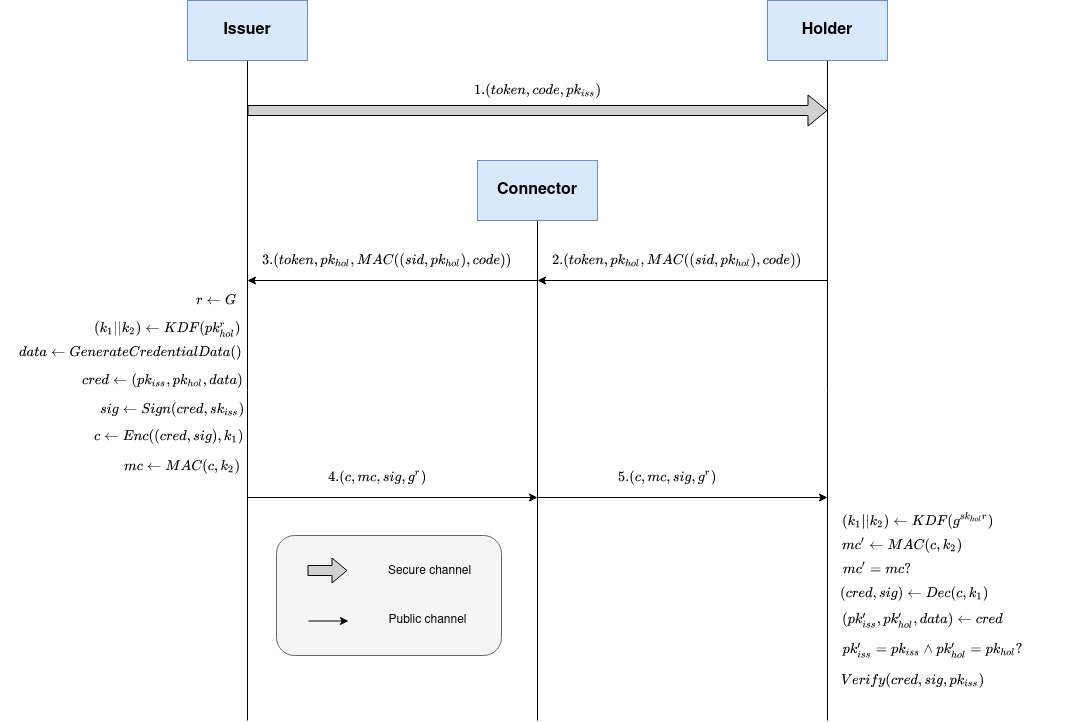
\includegraphics[scale=0.4]{figures/connector.png}
  \caption{Sequence diagram for the E2EE protocol through the connector.}
  \label{fig:e2econnector}%
\end{figure}

The security properties that we prove are as follows (we refer to the actual
model for the formal definition):

\begin{description}
\item[Code secrecy.] Codes exchanged via a QR code are always confidential.
  Note that this is trivial, as it is exchanged via a secure channel, and
  the holder never sends it back in the clear.
\item[Code injectivity.] Every QR code that is received by a holder, allegedly
  sent by an issuer, was sent before by that issuer. Again, this is trivial due
  to the secure channel used to exchange the QR code.
\item[Holder's public key authenticity.] Every message received by an issuer
  in step 3, containing a public key for key-exchange usage, that was
  allegedly sent by a holder, was indeed previously sent by that holder.
  This is ensured through the message authentication code (MAC) that
  leverages the random QR code exchanged via the secure channel, which is
  only known to the issuer and the holder.
\item[Holder's public key injectivity.] For every session in which an
  issuer receives in step 3 a message, allegedly sent by a holder in
  step 2, containing the holder's public key, it was that holder, in
  the same session, who sent the public key in step 2.  
\item[Credential secrecy.] This property has two variants: it ensures
  secrecy for credentials sent by an honest issuer to a holder that was honest
  at the moment of sending the credential, and is not compromised afterwards;
  and it also ensures secrecy for credentials received by an honest holder,
  allegedly from an honest issuer, if both holder and issuer were honest when
  the credential is received, and they are not corrupted afterwards. Altogether
  with the credential authenticity property shown next, it ensures that only
  (honest) holder and issuer learn the contents of a credential.
\item[Credential authenticity.] All messages containing a credential, received
  by a holder at step 5, where indeed sent by an issuer and addressed to that
  same holder, as long as both issuer and holder keys are not compromised.
\item[Credential non-injectivity.] All messages containing a credential, received
  by a holder at step 5, were sent by an issuer and addressed to that holder
  at step 4. Note, however, that both messages in steps 4 and 5 don't necessarily
  pertain to the  same ``session'' (in instantiations where parallel sessions
  may occur). However, our current understanding is that this does not pose a
  risk, as in any case, the messaged is sent by the issuer, and received by the
  intended holder. For the sake of future reference, we give an illustrative
  flow of this ``non-injective'' execution, in \appref{app:non-inj-e2ee}.
\end{description}

%----------------------------------------------------------------------------------------
%	PROPERTIES
%----------------------------------------------------------------------------------------

\section{Properties we believe we have}

\paragraph{Unforgeability.} A user cannot forge issuer-generated credentials.
\paragraph{Privacy against issuers.} An issuer does not learn whether a user (who acquired a credential from the issuer) has interacted with a given verifier (assuming no cooperation between issuer and verifiers).
\paragraph{Revocability.} An issuer can revoke a previously-issued credential without users’ cooperation.
\paragraph{Protection against credential reuse.} A verifier can ensure no credential is used by different DIDs. 
\paragraph{Deferred and offline verification checks.} A verifier can verify the revocation status of a credential asynchronously without users’ participation. A verifier can also verify a credential without contacting the internet, in which case the verification result is with respect to the last time the verifier synchronized with blockchain events.
\paragraph{Resistance to key rotation.} If an issuer's issuing key is revoked, credentials already issued by that key remain valid. This means that the issuer does not need to re-issue the credentials signed by a compromised issuing key. This is possible due to the fact that key revocation and credential issuances are timestamped. Hence, if an issuing key is revoked, credentials already issued remain valid unless they are explicitly revoked.
\paragraph{Independence of issuers and verifiers.} Verifiers only need to know which issuer DIDs they trust. They do not need to contact issuers to query issuance nor revocation lists.
\paragraph{Past preservation.} Any party that verifies a credential has non-reputable information of when the credential was valid even if it has been revoked.

\section{Properties we are not offering}

\paragraph{Unlinkability.} A coalition of verifiers cannot link activities of users across verifiers.
\paragraph{Minimal disclosure.} A user only reveals what is necessary to establish a relationship with a verifier.

%----------------------------------------------------------------------------------------
%	PROPOSED IDEAS
%----------------------------------------------------------------------------------------

% \section{Ideas to add missing properties}
\section{Further thoughts}

\subsection{Scaling} 

In the previous sections we described a protocol that allows transparent management of decentralized identifiers and credentials.
The protocol usage of a blockchain facilitates the solution to three points:
\begin{itemize}
\item Events ordering: All participants can agree on the order in which any pair of events occurred 
\item Fork protection (safety): There is no point in time where a valid sequence of processed protocol events could become invalid, nor replaced by 
      another sequence
\item Data transmission: All participants receive the same sequence of protocol events as they are transmitted through the blockchain
\end{itemize}

The second point has particular relevance to guarantee that the history of events can be trusted. For instance, imagine Alice controls a DID (its 
associated master keys) that represents a real world object, like a car. If Alice's wants to sell the car and transfer the corresponding DID, she 
would perform a DID update that revokes all the master keys controlled by her, and adds a new master key controlled by the new car owner. If Alice 
could later "undo" this update, the DID ownership transfer could not be trusted.

The properties brought by the blockchain come at a cost. Namely, the protocol throughput (number of events that participants can attach in 
transactions per unit of time) is bounded to the blockchain throughput. In order to scale the throughput, we have reviewed Sidetree's approach. The 
idea behind Sidetree is to not publish individual events attached to blockchain transactions, but to publish a hash-link to an off-chain content 
addressable storage (CAS), like IPFS. The CAS will contain the file referenced by the hash-link, which contains a batch of many protocol events 
(allowing to transcend the size limits imposed by blockchain transactions).

We identify a non-ideal drawback about this approach, which is a loss of the safety property. In the setting defined by Sidetree, participants can 
control changes to the past of their identifiers. This is, if Alice desires, she could create a DID by posting a file, $F_{1}$ on the CAS, and its 
hash on-chain, $F_{1}$ would contain Alice $CreateDID$ event. Later, Alice can create a file $F_{2}$, containing an $UpdateDID$ event, post the hash 
of $F_{2}$ on-chain, but intentionally not posting $F_{2}$ on the CAS. Then, Alice can create a third file $F_{3}$ which contains an new $UpdateDID$
event that would be invalid if $F_{2}$ were revealed in the CAS (e.g. $F_{2}$ event could revoke the key that signs the update in $F_{3}$). However, 
Alice can post both $F_{3}$ in the CAS and the hash of $F_{3}$ on-chain. In Sidetree, this sequence of actions would lead all protocol participants 
to believe that Alice's DID is in certain state, produced by the $CreateDID$ of $F_{1}$ and the $UpdateDID$ from $F_{3}$.

Alice has the power to reveal at any point $F_{2}$, making the update from $F_{3}$ as invalid, and forcing all participants to update Alice's
DID to the state reflected by $F_{2}$. This is known as \textbf{late publish attack}, and makes technically impossible to trust the past history 
history of events in Sidetree implementations. As an example consequence, it is not possible to transfer ownership of a DID when using Sidetree.

In order to avoid introducing this issue, we considered two options. 

The first one is to add a permissioned actor (or a federation of them) that are allowed to batch protocol events and publish both on-chain hash-links,
and files in corresponding CAS. The special actor introduces a trust model that assumes that it will always reveal files. If the actor fails to 
reveal a file, the protocol participants stop processing further batches until the missing file is revealed. This is not possible in Sidetree because
any participant would be able to freeze the system by not revealing a file. The protocol would still allow users to publish events on-chain directly, 
leaving space for some decentralization for those participants that do not want to depend on the centralized batcher. 

In order to use the batcher to publish the $UpdateDID$ events associated to a DID $D$, the owner of $D$ will have to declare on-chain that future 
updates for $D$ will be found on the off-chain batches. This public declaration is needed to avoid race conditions when a hash is on-chain but
a file is not revealed.

A second option consist of a more decentralized variation of the previous approach. Namely, allow any participant to propose itself as an event 
batcher. The proposal is performed by submitting an on-chain event declaring the batcher DID. Every user that would like to batch its events 
off-chain should publicly notify the batcher they will use. Only one batcher can be assigned to each DID, this is, the $UpdateDID$ events associated 
to a DID will be published by at most one batcher. The objective is once again, to be able to identify missing files in a sequence, allowing 
participants to stop processing files out of order. 

In any of the approaches, if the associated batcher stops publishing files, the DID registered to the batcher is "frozen" until the file is revealed.
We could re-introduce some liveness protection to DID owners by requesting batches from a same batcher to be separated at least $N$ underlying 
blockchain blocks, in order to provide that time for users to send a $Contention$ event that invalidates the events associated to a DID published in
the previous batch. During the processing of batches, participants will wait the contention period (the $N$ blocks) before applying events from a 
batch in order to not apply the updates to contended DIDs.

Notes:
\begin{itemize}
\item we could change the $CreateDID$ event to incorporate an optional batcher DID from start, the batcher DID would be part of the initial state, 
      bounding the batcher to the DID suffix. 
\item we could support events to de-register from a batcher, and to switch batcher too.
\item a user is free to batch his own DIDs' related events. This could be useful for a case like a car manufacturer that would like to batch all DIDs
      associated to their cars, allowing car owners to de-register from a batcher at will.
\item a priori, we do not see a need to batch credential issuance/revocation events
\end{itemize}

\appendix

\section{Example of Non-Injective Execution of Connector E2EE Protocol}
\label{app:non-inj-e2ee}

The diagram in \figref{fig:e2econnector-noninj} depicts an scenario in which a
non-injective execution between the issuer and the holder takes place.

First, we have to take into account that such execution requires a somehow
extended setting than what we considered in \secref{sssec:e2eeconnector}. Namely,
here we assume a (certainly realistic) scenario in which any prospective holder
has several computing devices -- e.g., a laptop and a smartphone. Similarly,
the issuer instantiates several concurrent services -- depicted as
\emph{Instance 1} and \emph{Instance 2} in \figref{fig:e2econnector-noninj}.
Still, the same user operates both computing devices, which share the same
private values; and all issuer instances have access to the same database with
holders' information, and the issuer's private keys.

\begin{figure}[ht!]
  \centering
  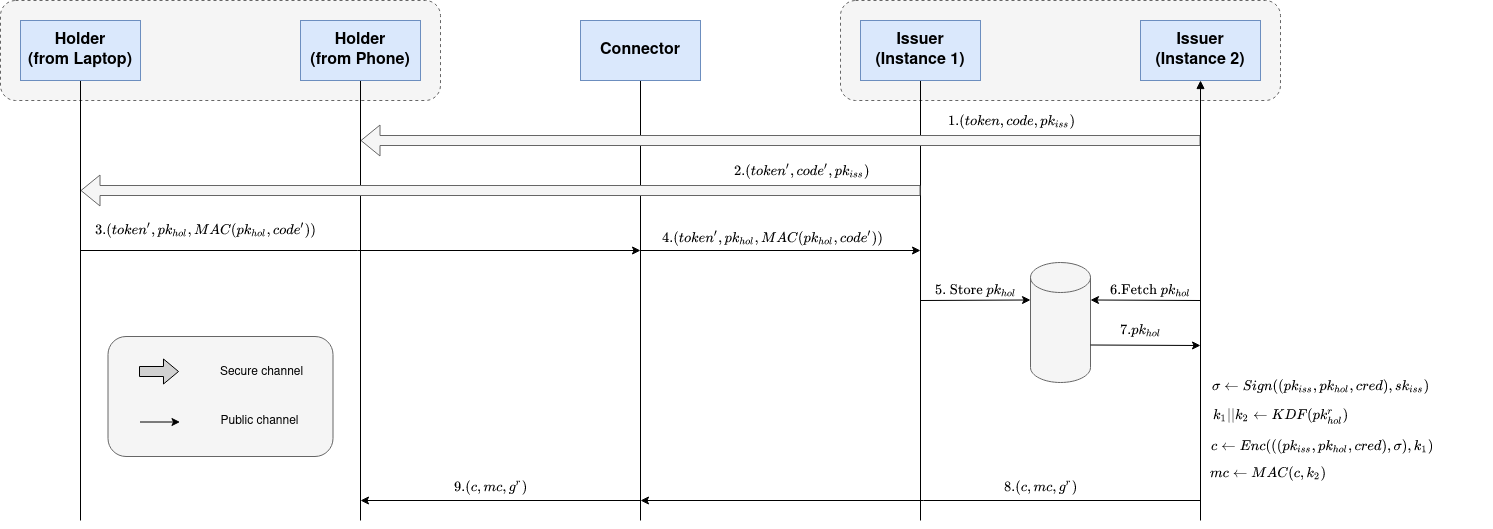
\includegraphics[scale=0.32]{figures/connector-noninjective.png}
  \caption{Sequence diagram of a sample non-injective execution of the E2EE
    connector protocol}
  \label{fig:e2econnector-noninj}%
\end{figure}

In the diagram, the holder requests a QR code once with each device -- for this,
we envision an extended setting in which the holder can request QR codes
securely (e.g., through signed email). The smartphone communicates with Instance
2 of the issuer, while the laptop communicates with Instance 1. Eventually, the
holder decides to complete the process from her laptop. The connector forwards
the request to Instance 1, which stores it in the database. Then, it might
happen that it is Instance 2 the one that takes care of finalizing the request:
it fetches the necessary data from the shared database, and sends the result to
the holder's phone (which is the computing device that communicated with
Instance 2). This lack of correspondence between who initiated a request, and
who responds it, is what is formally referred to as non-injectivity.
Theoretically, that might perfectly happen in our proposed protocol, as there is
nothing preventing such behaviour in a cryptographic manner, as our model shows.
However, two observations are relevant:

\begin{itemize}
\item The authenticity and secrecy properties still ensure that only the holder
  and issuer have access to the data that is sent by the issuer, and that it
  indeed originates from the issuer.
\item Such behaviour, if deemed unwanted, could be easily prevented through a
  proper session handling, at the implementation level.
\end{itemize}

\bibliographystyle{plain}
\bibliography{article}

\end{document}
